\documentclass[border=2pt]{standalone}
\usepackage{tikz}
\usepackage{amsmath}
\usepackage{mathtools}
\usetikzlibrary{arrows.meta,chains,%
                    decorations.pathreplacing}
\usetikzlibrary{matrix,positioning,arrows.meta,arrows}
\usetikzlibrary{shapes.geometric}
\usetikzlibrary{shapes.misc}

\newcommand\hlight[1]{\tikz[overlay, remember picture]\node[rectangle,fill=blue!50,rounded corners=0.5em,fill opacity = 0.2,draw,thick,text opacity =1] {$#1$};} 

\newcommand\hhlight[1]{\tikz[overlay, remember picture]\node[rectangle,fill=red!50,rounded corners=0.8em,fill opacity = 0.2,dashed,text opacity =1] {$#1$};} 

\tikzset{
mymat/.style={
  matrix of nodes,
  nodes in empty cells,
  text height=2.5ex,
  text depth=0.75ex,
  text width=3.25ex,
  align=center,
  column sep=-\pgflinewidth
  }
}
\tikzset{
  rows/.style 2 args={
    sub@rows/.style={row ##1 column #2/.style={nodes={rectangle,draw=black}}},
    sub@rows/.list={#1}
  },
  box/.style 2 args={
    sub@box/.style={rows={#1}{##1}},
    sub@box/.list={#2}
  }
}
\begin{document}

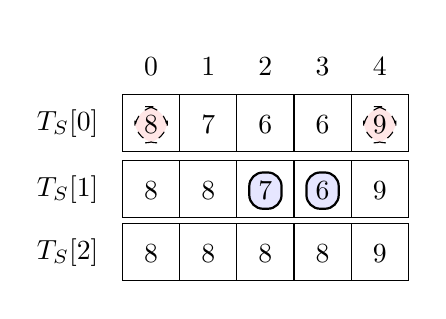
\begin{tikzpicture}[>=latex]

\matrix[mymat,anchor=west,
    box={2}{1, 2, 3, 4, 5}]
at (0,-3.5) 
(sp-mat1)
{ 
  0 & 1 & 2 & 3 & 4 \\
  \hhlight{8} & 7 & 6 & 6 & \hhlight{9}\\ };

  \matrix[mymat,anchor=west,
    box={1}{1, 2, 3, 4, 5}]
at (0,-4.7) 
(sp-mat2)
{ 
  8 & 8 & \hlight{7} & \hlight{6} & 9\\ };

\matrix[mymat,anchor=west,
    box={1}{1, 2, 3, 4, 5}]
at (0,-5.5) 
(sp-mat3)
{ 
  8 & 8 & 8 & 8 & 9 \\ };

\node[left=5pt of sp-mat1-2-1.west]{ $T_S[0]$ };

\node[left=5pt of sp-mat2-1-1.west]{ $T_S[1]$ };

\node[left=5pt of sp-mat3-1-1.west]{ $T_S[2]$ };

% \node[right=5pt of mat1]
% {
%   $T_s[i][j] = \left\{\begin{matrix*}[l]
%     \max(B_{j+1}) && , i = 0\\
%     \max(T_s[i-1][j], T_s[i-1][j-2^{i-1}]) && , \textit{otherwise}
%   \end{matrix*}\right.$
% };

% \node[right=5pt of mat2]
% {
%   $SQ_L = T_s[1][2] = 7$
% };

% \node[right=5pt of mat3]
% {
%   $SQ_R = T_s[1][3] = 6$
% };

\end{tikzpicture}

\end{document}